\documentclass{beamer}
\usepackage[french]{babel}
\usepackage[utf8]{inputenc}
\usepackage[T1]{fontenc}
\usetheme{Antibes}
\begin{document}
\title{Hôtel à insectes}
\subtitle{Intégration urbanistique}
\author{Alexandre Dulaunoy}
\maketitle
\begin{frame}{Agenda}
    \begin{itemize}
        \item{Objectif des hôtels à insectes}
        \item{Structure et construction}
        \item{Intégration dans un milieu urbain}
        \item{Bibliographie}
    \end{itemize}
\end{frame}
\begin{frame}{Objectif}
    \begin{itemize}
        \item Reconstruire l'habitat naturel des guêpes et abeilles sauvages
        \item $\rightarrow$ raréfaction des {\bf abris} (destruction des haies, façades lisses des maisons, nettoyage excessif)
        \item $\rightarrow$ raréfaction de la {\bf nourriture} (diminution des friches, de la culture extensive, des fleurs sauvages et des pelouses sauvages)
        \item $\rightarrow$ modification du {\bf paysage} (diminution des espaces mixtes, déstructuration des couloirs ecologiques)
    \end{itemize}
\end{frame}

\begin{frame}{Structure et Construction}
        \begin{itemize}
                \item La seule limite est votre créativité
        \end{itemize}
\end{frame}
\begin{frame}
        \includegraphics[scale=0.05]{./exemples/large.jpg}
\end{frame}
\begin{frame}
        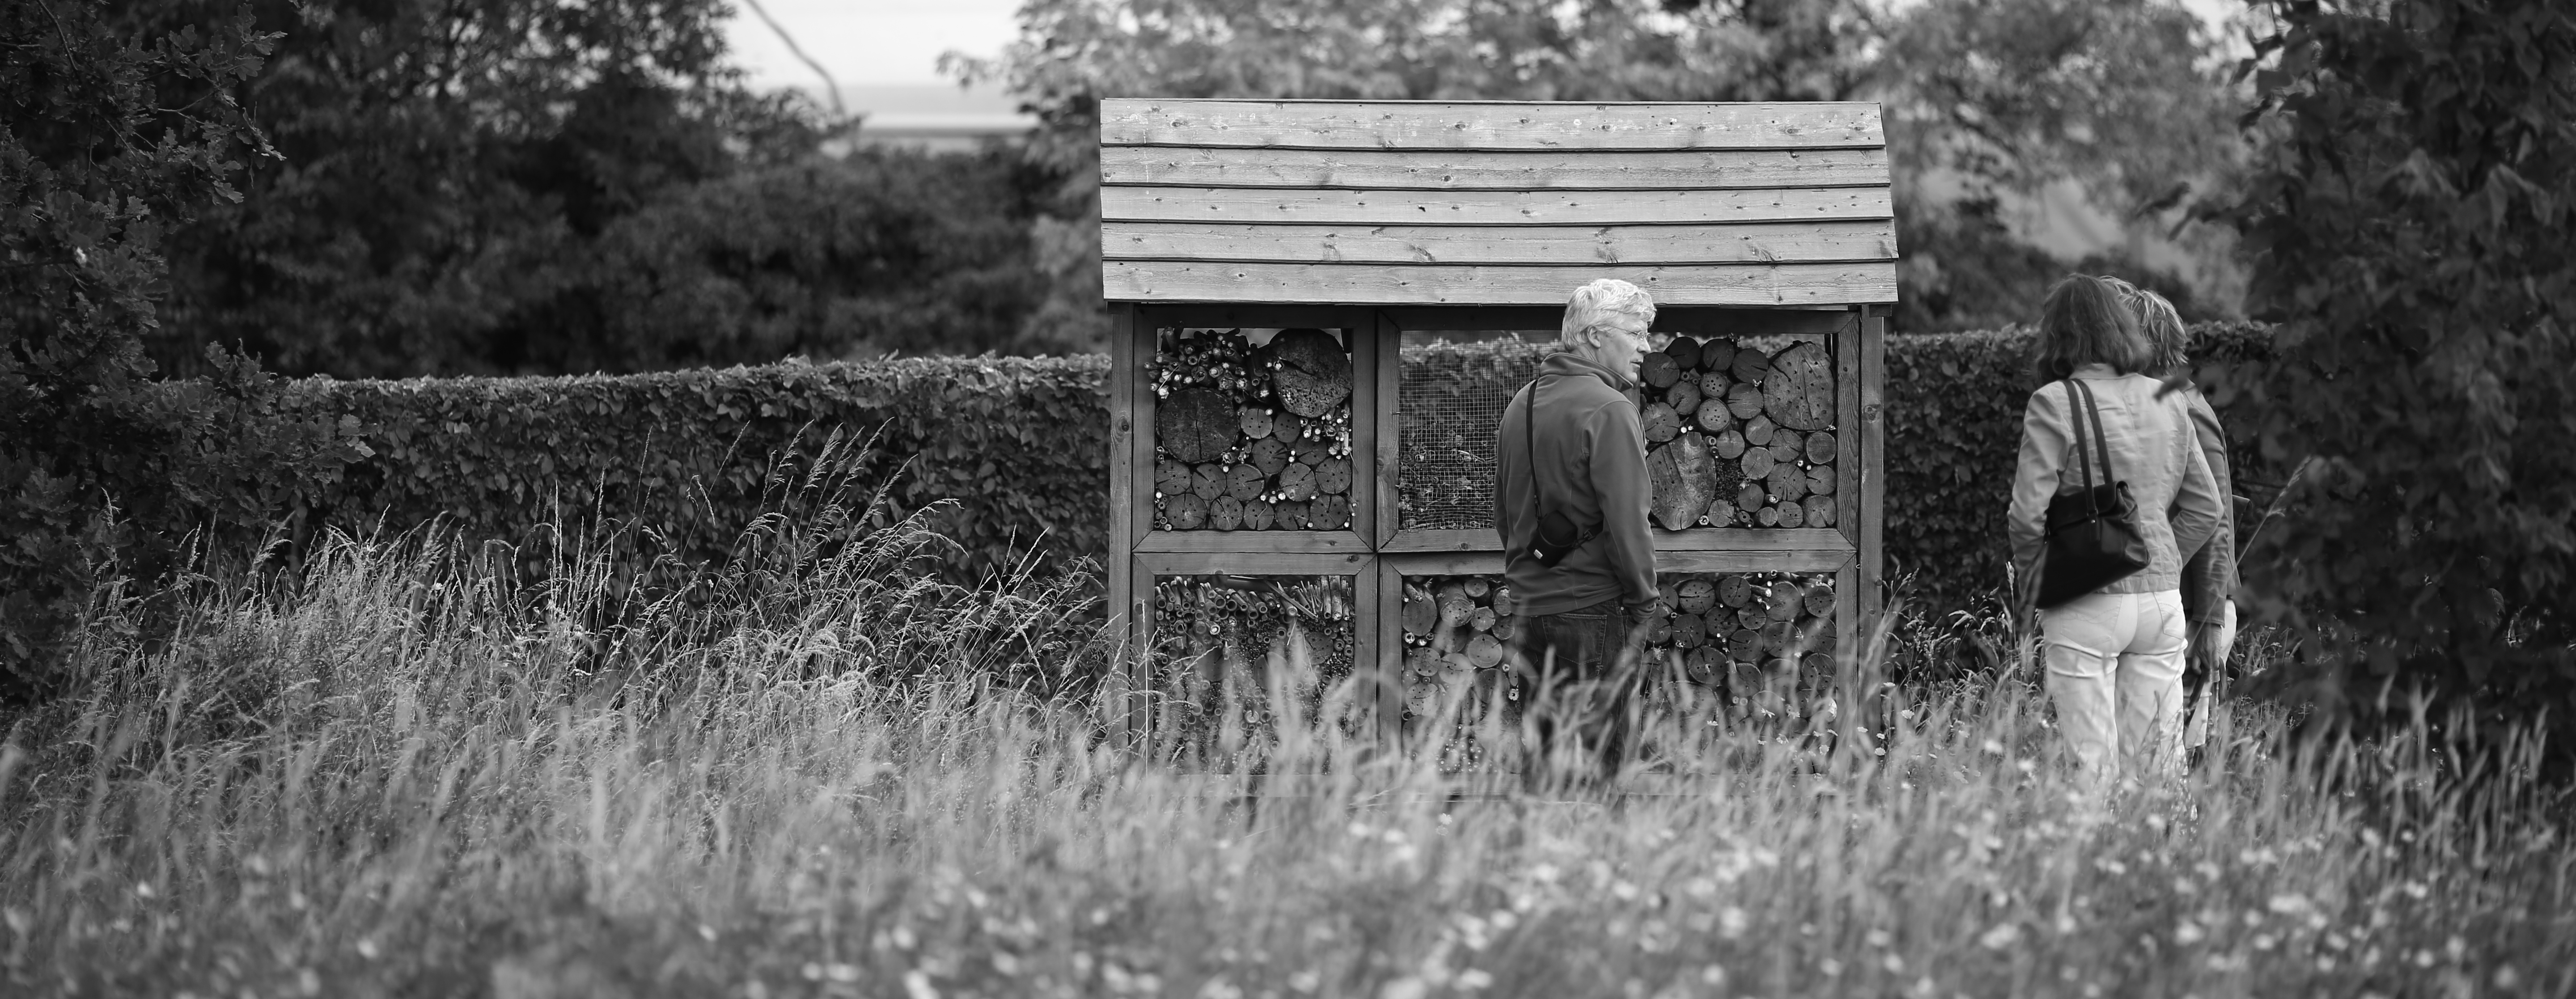
\includegraphics[scale=0.05]{./exemples/integration.jpg}
\end{frame}

\begin{frame}
        \includegraphics[scale=0.04]{./exemples/hotel-osmies.jpg}
\end{frame}
\begin{frame}
        \includegraphics[scale=0.04]{./exemples/pal.jpg}
\end{frame}
\begin{frame}
        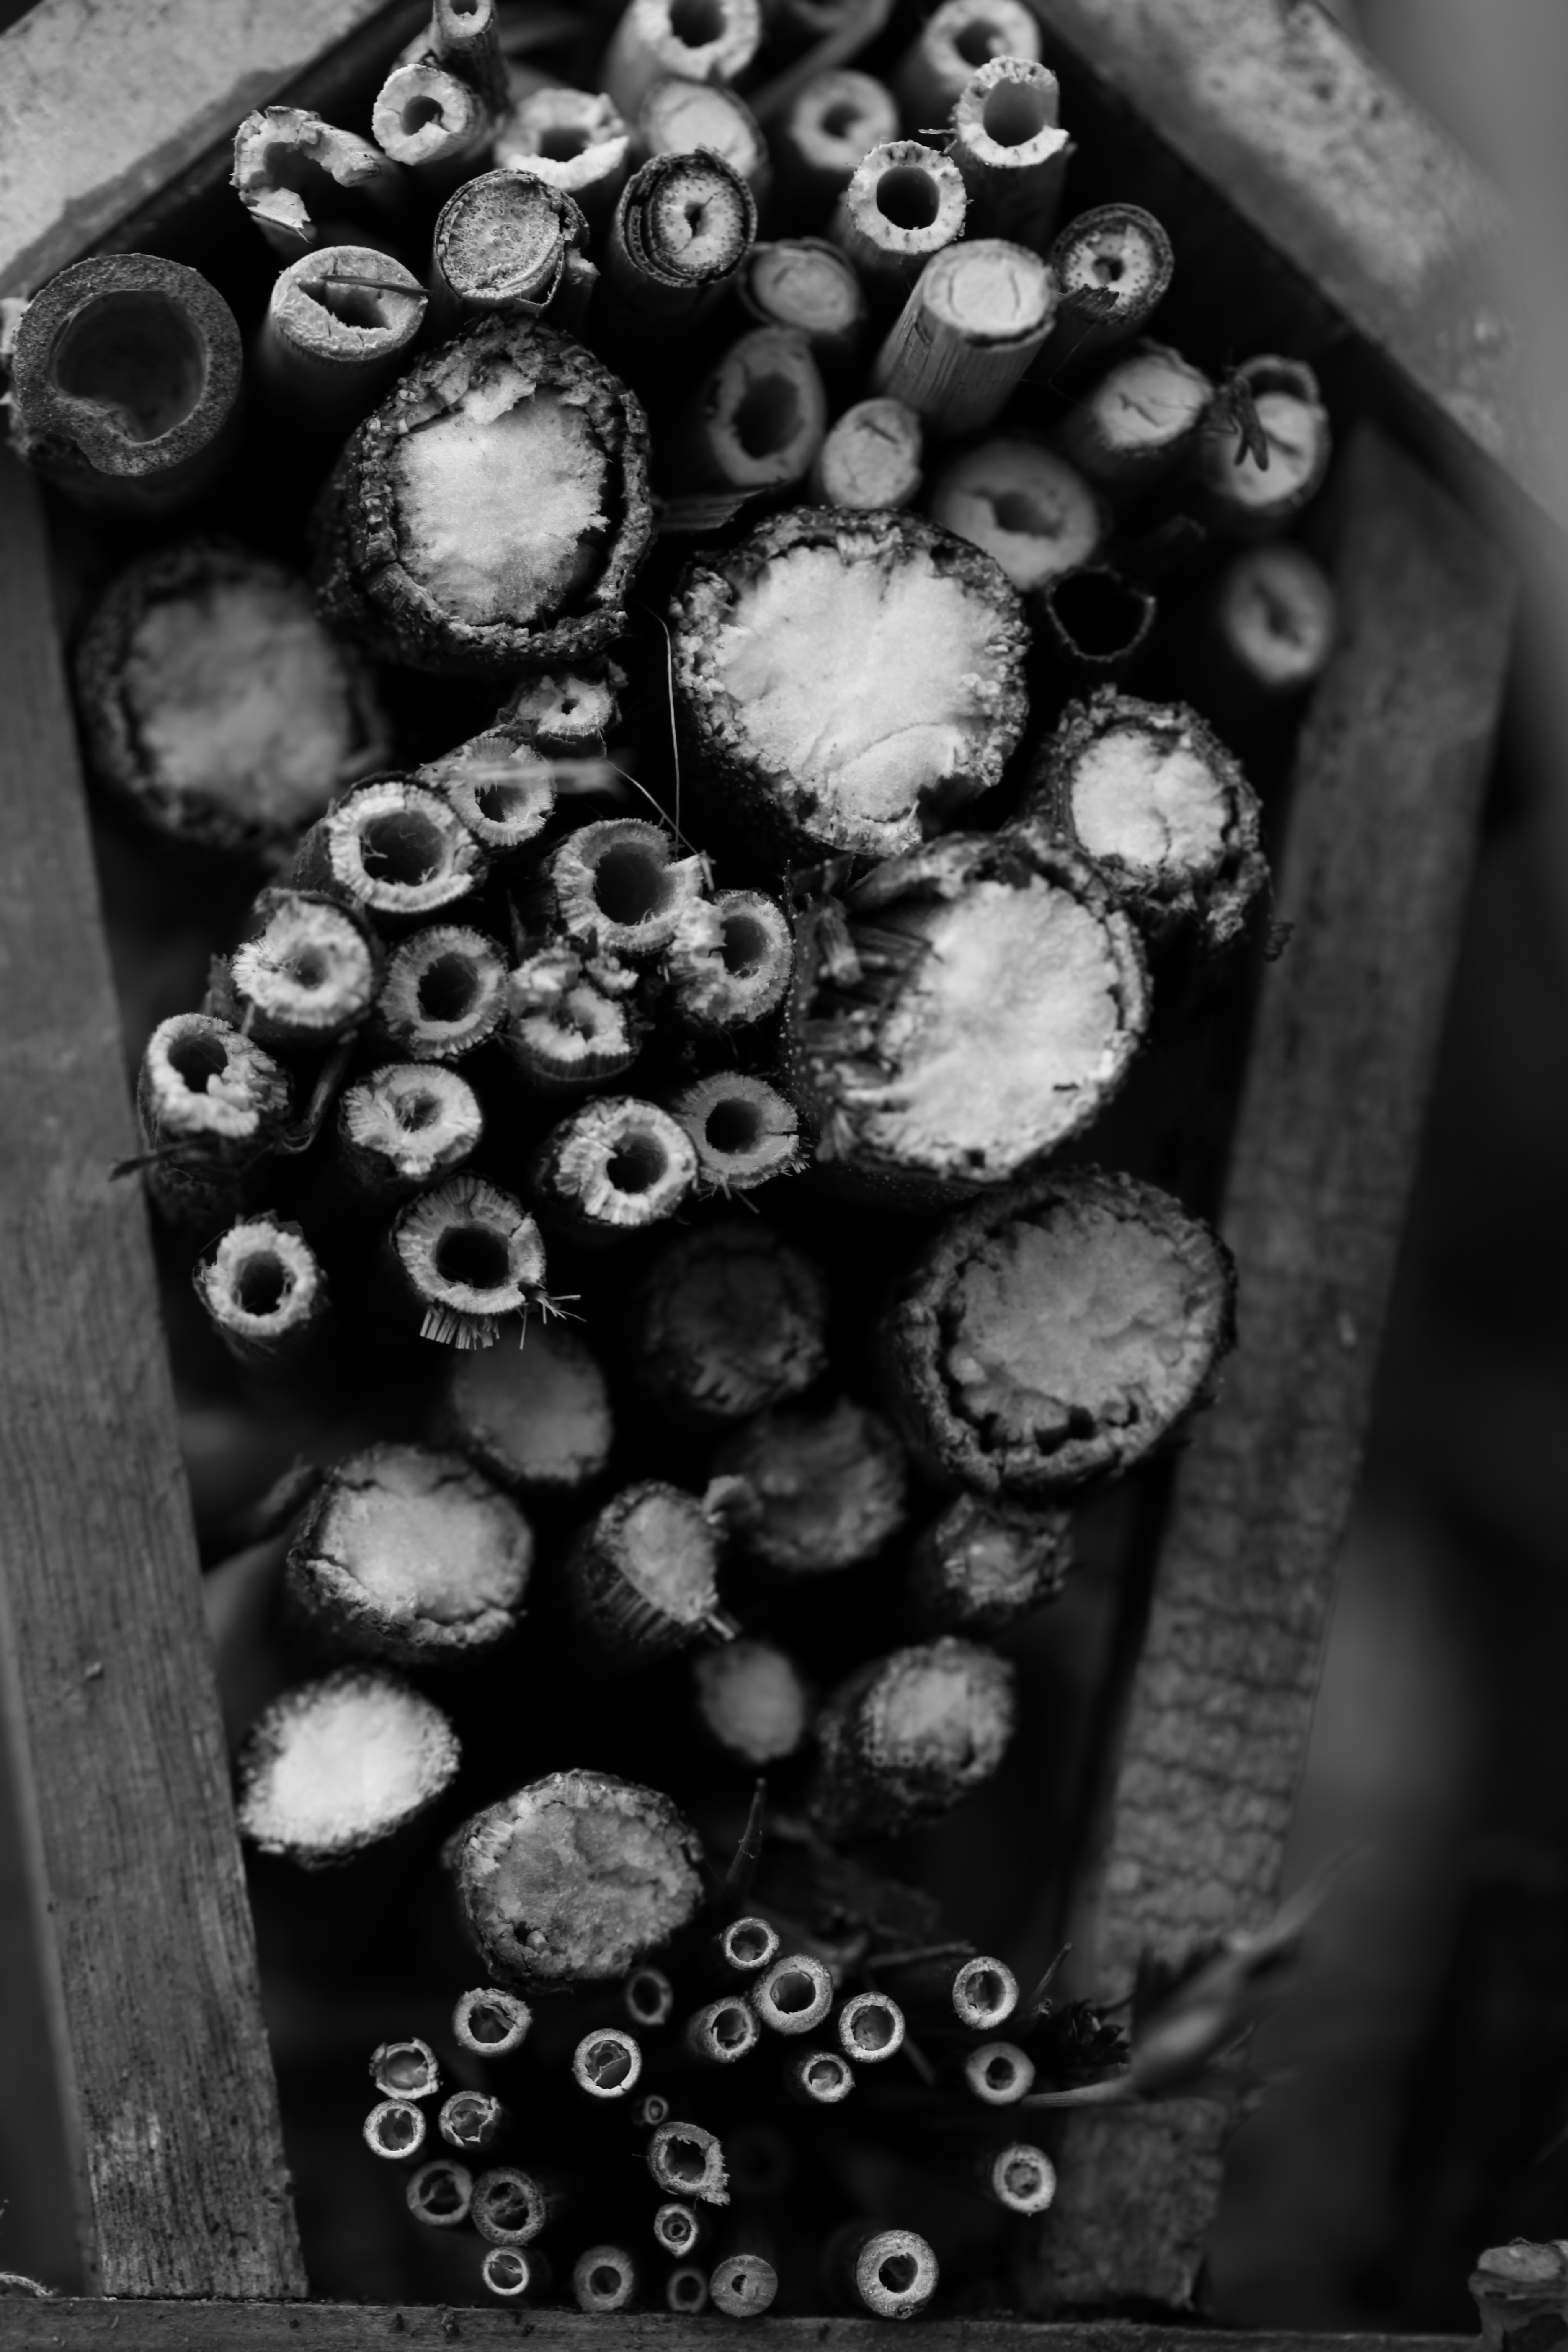
\includegraphics[scale=0.04]{./exemples/tige-moelle.jpg}
\end{frame}



\begin{frame}{Intégration dans un milieu urbain}
        \begin{itemize}
                \item La règle principale est l'orientation des hôtels à insectes : {\bf sud et face au soleil}
                \item Dos aux vents dominants et/ou courant d'air
                \item Abrité des intempéries (règle pour une majorité des insectes mais pas tous)
                \item Au minimum à 40 centimètres du sol
                \item Nourriture à disposition (fleurs sauvages mais n'oubliez pas qu'une partie des insectes sont aussi carnivores)
        \end{itemize}
\end{frame}

\begin{frame}{Bibliographie}
        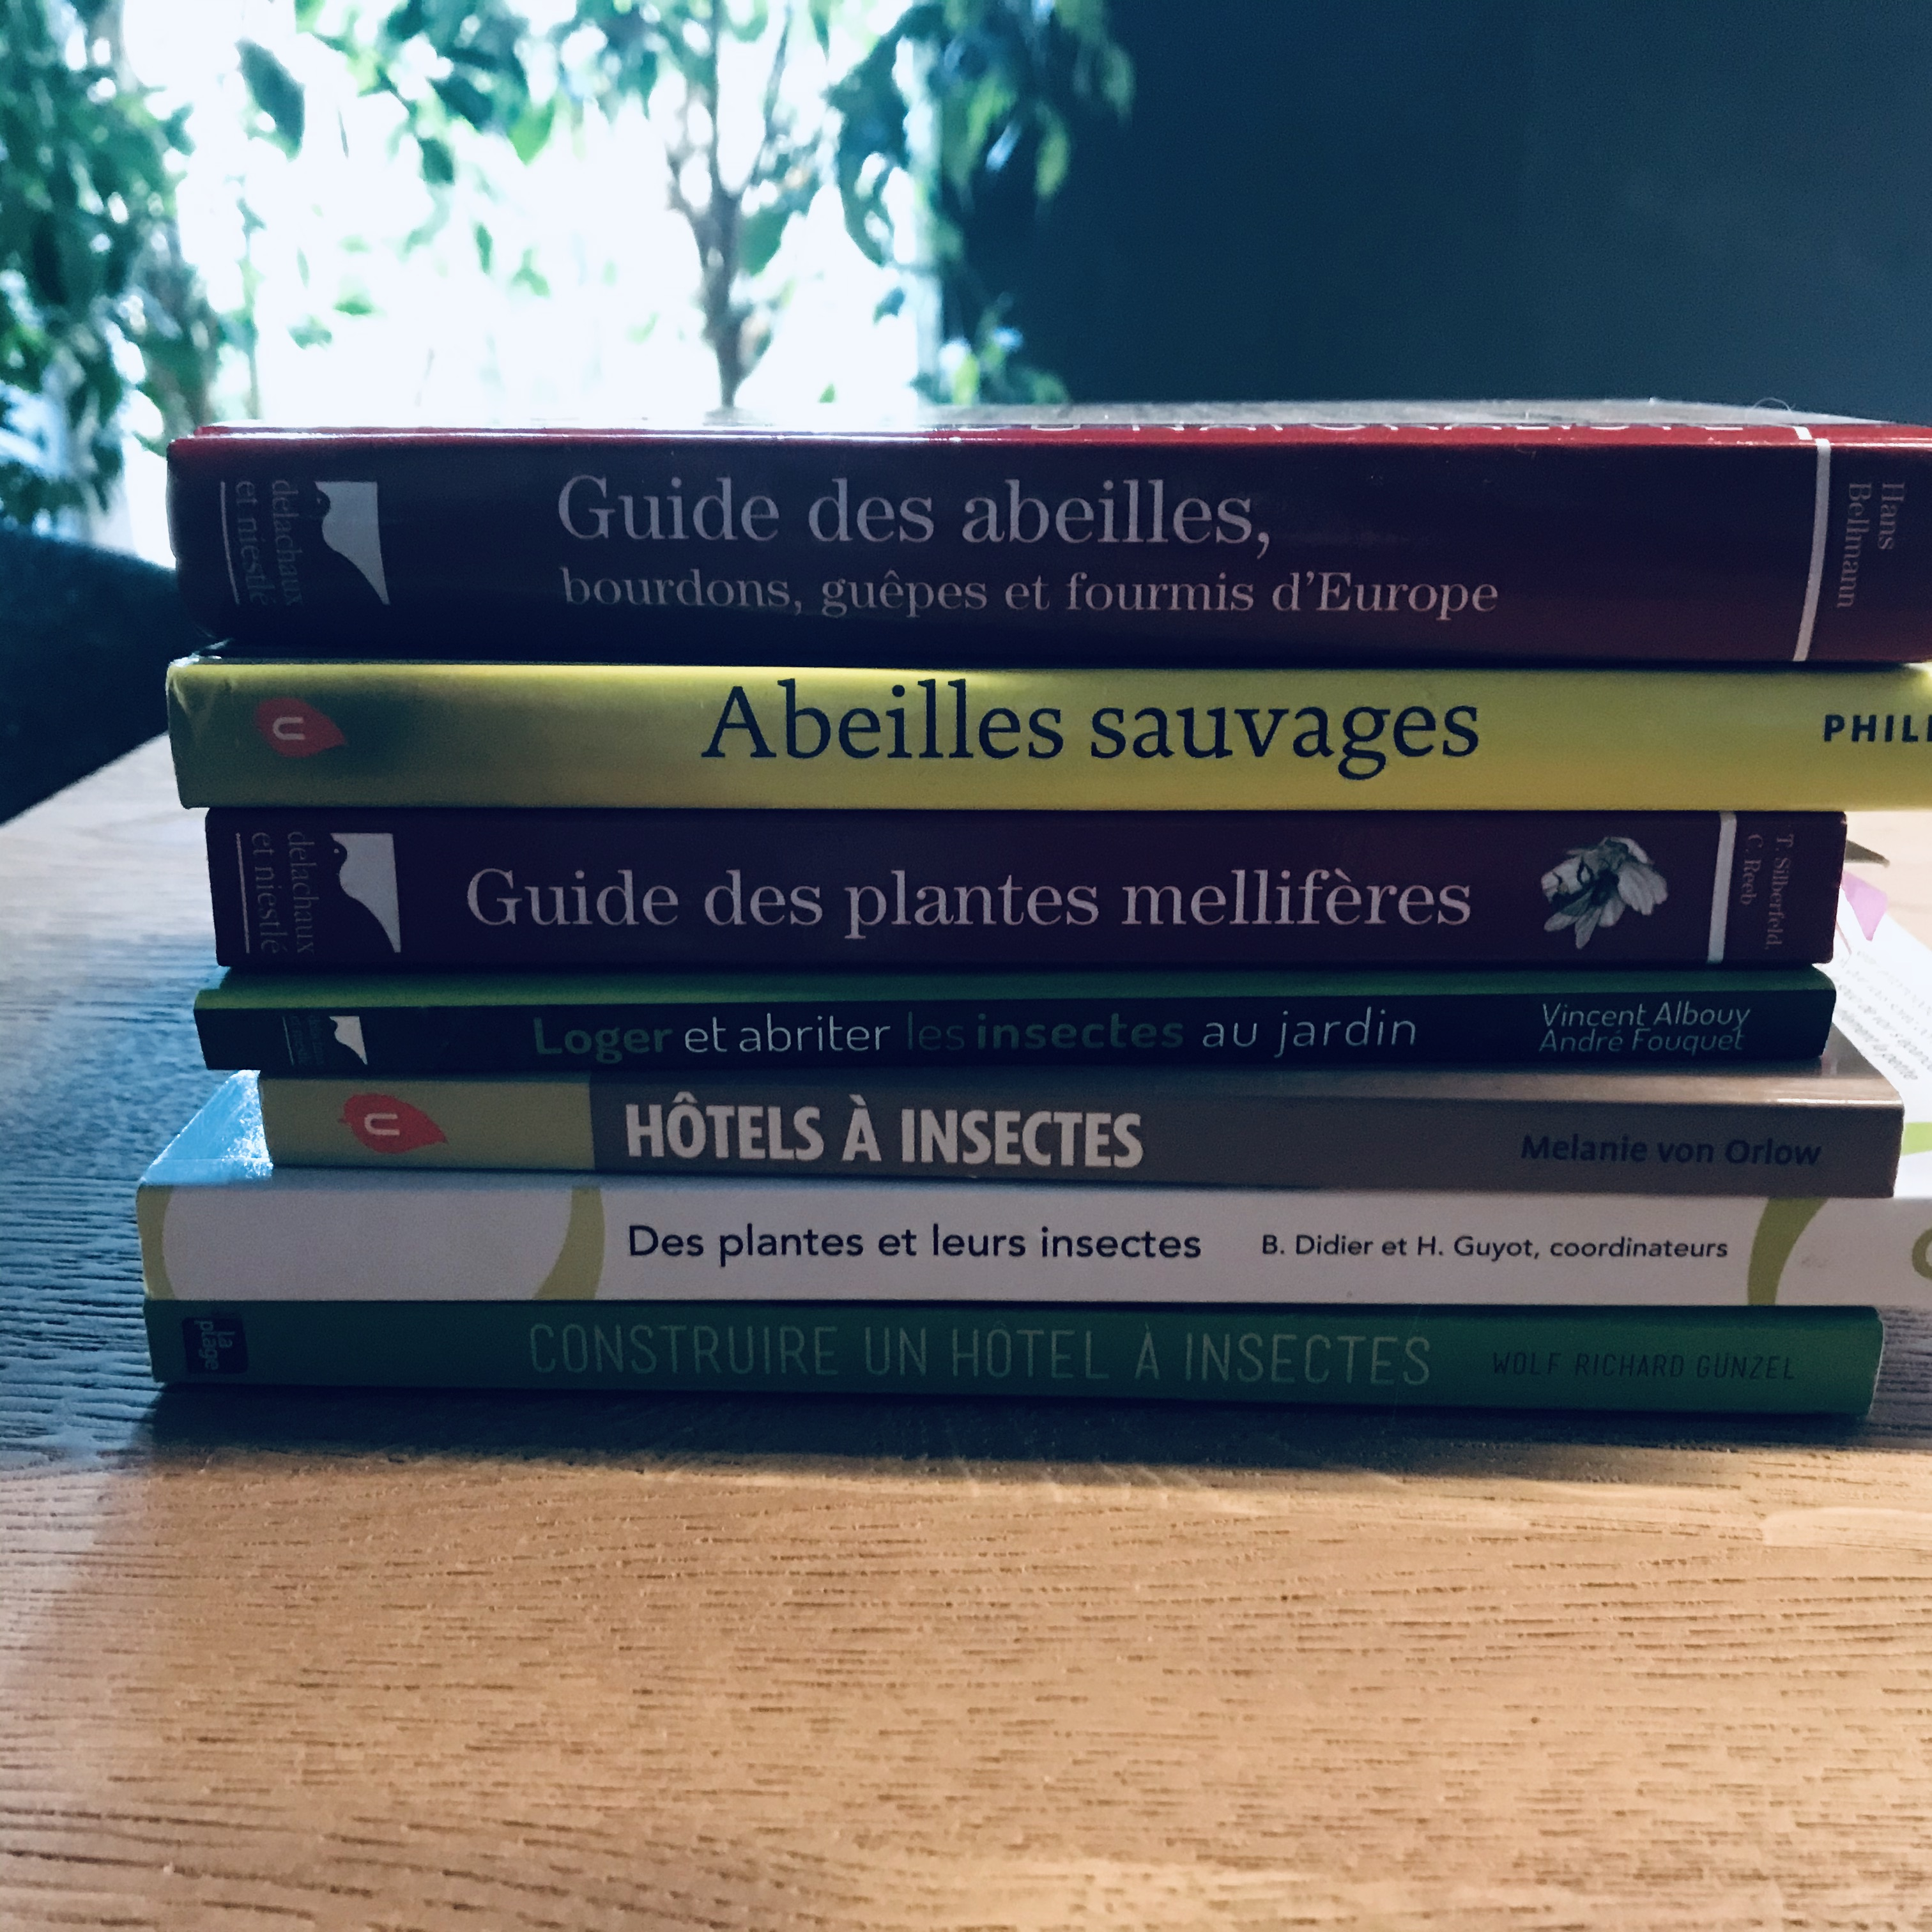
\includegraphics[scale=0.09]{./exemples/biblio.jpg}
\end{frame}

\end{document}


